\documentclass[english,twoside, openright, hidelinks, 11 pt, class=report,crop=false]{standalone}
\input{../preamb}
\input{bm}

%\renewcommand*\familydefault{\sfdefault} % For dyslexia-friendly text

% Norwegian names of figures, chapters, parts and content
\addto\captionsenglish{\renewcommand{\figurename}{Figur}}
\makeatletter
\addto\captionsenglish{\renewcommand{\chaptername}{Kapittel}}
\addto\captionsenglish{\renewcommand{\contentsname}{Innhold}}


\begin{document}
	
	\pagecolor{blue!20}
	
	\begin{titlepage}
		\begin{center}
			\vspace*{1cm}
			
			{\fontsize{25}{30}{\textbf{Teoretisk matematikk 2} \\[12pt]
		}}
			
			\vspace{2.45cm} 
			\begin{figure}[H]
				\centering
				\qquad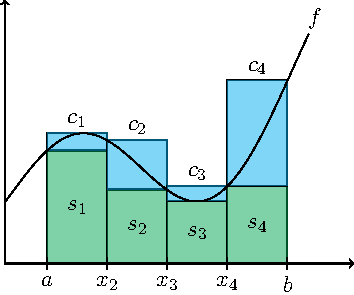
\includegraphics[scale=1.8]{fig/frpg}
			\end{figure}           
			\vspace{2 cm}
			\raggedleft Sindre Sogge Heggen   \end{center}
	\end{titlepage}
	\pagecolor{white}
\newpage
\phantom{}
\thispagestyle{empty}	
\newpage	
\import{kap0/}{forord}
\newpage

%\addcontentsline{toc}{chapter}{Innhold}
\footnotesize
\tableofcontents
\normalsize
\chapter{Følger og rekker\label{Folgerogrekker}}
\vspace{20pt}
\import{fol/}{fol_bm}
\newpage
\import{fol/}{fol_opg_bm}

\chapter{Trigonometri\label{Trigonometri}}
\vspace{20pt}
\import{tri/}{tri_bm}
\newpage
\import{tri/}{tri_opg_bm}
\newpage
\import{tri/}{cmt}

\chapter{Vektorer i rommet\label{Vektorerirommet}}
\vspace{20pt}
\import{vek/}{vek_bm}
\newpage
\import{vek/}{vek_opg_bm}

\chapter{Romgeometrier\label{Romgeometrier}}
\vspace{20pt}
\import{rom/}{rom_bm}
\newpage
\import{rom/}{rom_opg_bm}

\chapter{Integrasjon \label{Integrasjon}}
\vspace{20pt}
\import{int/}{int_bm}
\newpage
\import{int/}{int_opg_bm}

\titleformat{\chapter}[hang]
{\normalfont\LARGE\bfseries}{}{}{\vspace{-1cm}\Huge}
\chapter*{Vedlegg \ref{husksincos}-\ref{intleibn} \label{Tips} \addcontentsline{toc}{chapter}{Vedlegg A-F}}
\phantomsection
\vspace{20 pt}
\import{tips/}{tips}
{\printindex \addtocontents{toc}{\protect\vspace{-5pt}}
	\addcontentsline{toc}{chapter}{Indeks}\phantomsection}
\chapter*{Fasit}
\setlength{\parskip}{5pt}
\addtocontents{toc}{\protect\vspace{-5pt}}
\addcontentsline{toc}{chapter}{Fasit}\phantomsection

{\footnotesize
\import{fol/}{fol_fas}
\import{tri/}{tri_fas}
\import{vek/}{vek_fas}
\import{rom/}{rom_fas}
\import{int/}{int_fas}
}
\phantom{}
\newpage
\thispagestyle{empty}
\phantom{}
\newpage
\import{kap0/}{bakside}
%\thispagestyle{empty} 
%\phantom{}
\end{document}
%\end{document}











